\documentclass[journal]{IEEEtran}

\usepackage{graphicx}
\usepackage{float}
\usepackage{amsmath}
\usepackage{algorithm}
\usepackage[noend]{algpseudocode}
\usepackage{mathtools}
\usepackage{multirow}
\DeclarePairedDelimiter\floor{\lfloor}{\rfloor}

\renewcommand\refname{Daftar Pustaka}
\renewcommand{\figurename}{Gambar}
\renewcommand{\tablename}{Tabel}

\begin{document}
	
\title{Kompresi Data pada Laporan Cuaca Menggunakan Metode \textit{Huffman Coding}}

\author{
	IF 38-01\\
	\vspace{1mm}
	Aliya Nur Rezkita\hspace{1.05cm} 1301144161\\
	Febby Febriansyah\hspace{1cm} 1301140371\\	
	Rizkiyana Prima Putra\hspace{0.4cm} 1301140181\\
	Tari Lestari\hspace{2.15cm} 1301144281\\
	\vspace*{1mm}
	Fakultas Informatika, Telkom University, Bandung\\
	Kontak : 082240203610 (Rizkiyana Prima Putra)
}

\markboth{Tugas Besar Dasar Pemodelan dan Simulasi IF 38-01}%
{Shell}

\maketitle
\renewcommand{\abstractname}{Abstrak}
\begin{abstract}
Sebuah instansi pengamat cuaca memiliki beberapa alat yang dapat memprediksi kemungkinan cuaca yang akan terjadi setiap harinya. Kemungkinan cuaca yang dapat diprediksi diantaranya cerah, berawan, hujan, dan berkabut. Hasil dari setiap sejumlah $n$ observasi yang dilakukan akan ditransmisikan ke server utama. Namun, permasalahnnya adalah ketika banyaknya alat yang digunakan akan mengakibatkan komunikasi transmisi data menjadi \textit{overload}. Sehingga diperlukanlah suatu metode yang dapat mengkompresi data ke dalam ukuran yang lebih kecil. Pada paper ini kami menggunakan metode \textit{Huffman Code} untuk meng-\textit{encoding} 4 nilai probabilitas cuaca menjadi deretan bit yang unik agar proses transmisi data menjadi lebih efisien.
\end{abstract}

\renewcommand{\IEEEkeywordsname}{Kata Kunci}
\begin{IEEEkeywords}
Kompresi data, Algoritma Huffman, Laporan Cuaca, Probabilitas.
\end{IEEEkeywords}
\vspace{1mm}
\renewcommand{\abstractname}{Abstract}
\begin{abstract}
	A weather forecaster has several tools that can predict the possible weather that will occur each day. That possible weather conditions are sunny, cloudy, rainy, and foggy. The results of each $ n $ observation will be transmitted to the main server. However, the problem is when the number of tools used will make data transmission communication becomes \ textit {overload}. So we need a method that can compress data into smaller sizes. In this paper we use the \ textit {Huffman Code} method to  encode the 4 weather probability values ​​into unique bit sequences to make data transmission more efficient.
\end{abstract}
\renewcommand{\IEEEkeywordsname}{Keywords}
\begin{IEEEkeywords}
	Data Compression, Huffman Coding, Weather Report, Probability.
\end{IEEEkeywords}


\section{Pendahuluan}
\hspace*{0.3cm}Banyak kegiatan atau aktifitas manusia yang bergantung pada faktor cuaca. Faktor cuaca ini terkadang memiliki pengaruh yang sangat besar bagi keberlangsungan kegiatan yang dilakukan. Peran seorang prakiawan cuaca sangat dibutuhkan mengingat cuaca adalah kondisi udara yang berlangsung dalam jangka waktu yang singkat, maka proses prakiraan cuaca jangka pendek harus dilakukan secara cepat dan seakurat mungkin. Kondisi cuaca di suatu tempat ditentukan oleh sejumlah faktor diantaranya temperatur udara, kelembaban udara, arah angin, kecepatan angin dan sebagainya. Dengan melihat faktor-faktor ini, seorang prakiawan cuaca dapat memprediksikan kondisi cuaca yang akan berlangsung pada keesokan harinya.\\
\hspace*{0.6cm}Berbagai metode dilakukan untuk memperoleh hasil informasi cuaca yang akurat, salah satunya menggunakan pendekatan model cuaca numerik. Perkembangan model cuaca numerik seiring dengan perkembangan kemampuan komputasi dan penambahan jaringan pengamatan telah mencapai akurasi prediksinya yang baik dan sudah banyak digunakan dalam membuat prakiraan cuaca oleh pusat layanan cuaca di banyak negara. Pola cuaca yang berbeda antar wilayah, mengharuskan dilakukan pengujian model cuaca numerik seperti pemilihan skema parameterisasi, syarat awal, waktu “spin-up” agar mampu menghasilkan prediksi yang terbaik~\cite{1}.\\
\hspace*{0.6cm}Namun, penggunaan model numerical melibatkan perhitungan parameter cuaca yang cukup banyak, umumnya prakiraan cuaca yang menggunakan metode ini mempunyai keluaran (file output) yang cukup besar. Besar kecilnya hasil keluaran ditentukan oleh beberapa faktor, antara lain: luas daerah yang diprediksi, panjang prediksi, resolusi spasial yang digunakan, dan parameter cuaca yang dihasilkan~\cite{2}.\\
\hspace*{0.6cm}Untuk Kota Bandung yang mempunyai wilayah yang cukup luas, penggunaan metode numerical ini akan memberikan permasalahan yang cukup signifikan dalam hal distribusi dan penyimpanan data-data prediksi cuaca. Ditambah lagi penggunaan dynamical downscaling (perolehan informasi spasial cuaca yang lebih detil/resolusi tinggi) untuk peningkatan akurasi prakiraan yang akan semakin memperbesar ukuran file output. Oleh karena itu, dibutuhkan suatu proses pengubahan sekumpulan data menjadi suatu bentuk kode untuk menghemat kebutuhan tempat penyimpanan dan waktu untuk transmisi data.\\
\hspace*{0.6cm}Dalam paper ini, pengubahan bentuk data menjadi kode, penulis akan menggunakan Algoritma Huffman yaitu algoritma dimana setiap nilai-nilai probabilitas masing-masing cuaca dikodekan hanya dengan rangkaian beberapa bit, dimana nilai yang sering muncul dikodekan dengan rangkaian bit yang pendek dan nilai yang jarang muncul dikodekan dengan rangkaian bit yang lebih panjang sehingga akan mempermudah untuk menyelesaikan suatu masalah perkiraan cuaca.\\
\vspace*{2cm}
\section{Metode Penelitian}
	\hspace*{0.3cm}Tahapan penelitian yang akan dilakukan dalam paper ini adalah menggunakan algoritma Huffman untuk pengubahan sekumpulan data menjadi suatu bentuk kode agar menghemat kebutuhan tempat penyimpanan dan waktu transmisi data.\\
\\
\textbf{\textit{Algoritma Huffman}}\\
\hspace*{0.7cm}Algoritma Huffman adalah salah satu algoritma kompresi. Algoritma huffman merupakan algoritma yang paling terkenal untuk mengompres data. Terdapat tiga fase dalam menggunakan algoritma Huffman untuk mengompres sebuah data, pertama adalah fase pembentukan pohon Huffman (\textit{tree}), kedua fase encoding dan ketiga fase decoding. Prinsip yang digunakan oleh algoritma Huffman adalah data yang sering muncul di-encoding dengan rangkaian bit yang pendek dan data yang jarang muncul di-encoding dengan rangkaian bit yang lebih panjang. Teknik kompresi algoritma Huffman mampu memberikan penghematan pemakaian memori sampai 30\%. Algoritma Huffman mempunyai kompleksitas $O(n log n)$ untuk himpunan dengan $n$ data~\cite{3}.\\
\\
Langkah-langkah pembentukan pohon Huffman adalah sebagai berikut :
\vspace*{0.5cm}
\begin{algorithm}[H]
	\caption{Algoritma Huffman}\label{alg:huffman}
	\begin{algorithmic}[1]
		\State Baca semua nilai di dalam himpunan data cuaca untuk menghitung frekuensi kemunculan setiap nilainya. Setiap nilai dinyatakan sebagai pohon bersimpul tunggal. Setiap simpul di-assign dengan frekuensi kemunculan nilai tersebut.
		\State Terapkan strategi algoritma sebagai berikut, gabungkan dua buah pohon yang mempunyai frekuensi terkecil pada sebuah akar. Setelah digabungkan, akar tersebut akan mempunyai frekuensi yang merupakan jumlah dua buah pohon-pohon penyusunnya.
		\State Ulangi langkah 2 sampai hanya tersisa satu buah pohon Huffman. Agar pemilihan dua pohon yang akan digabungkan berlangsung cepat, maka semua pohon yang ada selalu terurut menaik berdasarkan frekuensi.
	\end{algorithmic}
\end{algorithm}
\vspace*{0.5cm}
\hspace*{0.3cm}Proses encoding untuk satu data dimulai dengan membuat pohon Huffman terlebih dahulu. Setelah itu, kode untuk satu data disusun sebagai biner yang dibaca dari akar sampai ke daun pohon Huffman.\\
\\
Langkah-langkah untuk melakukan encoding pada suatu data adalah sebagai berikut :
\begin{algorithm}[H]
	\caption{Encoding} \label{alg:encoding}
	\begin{algorithmic}[1]
		\State Tentukan data yang akan di-encode.
		\State Mulai dari akar, baca setiap bit yang ada pada cabang yang bersesuaian sampai menemukan daun di mana data itu berada.
		\State Ulangi langkah 2 sampai seluruh data di-encode.
	\end{algorithmic}
\end{algorithm}
\section{Simulasi}
\textbf{\textit{Flowchart}}\\
\begin{figure}[H]
		\centering
		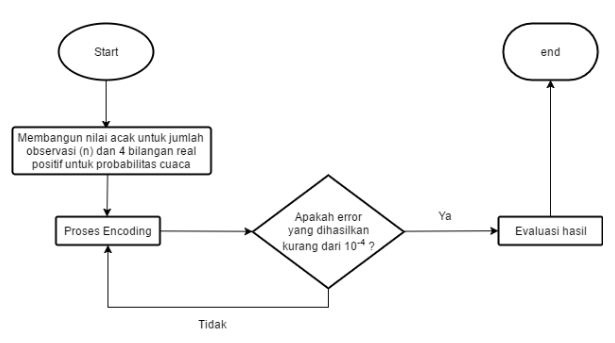
\includegraphics[width=\linewidth]{Capture2.png}
		\caption{Flowchart}
		\label{fig:flowchart}
\end{figure}
\textbf{\textit{Input Simulasi}}\\
\hspace*{0.6cm}Input simulasi pada kasus Weather Report ini adalah dua baris yang terdiri atas jumlah observasi $N$ dengan interval $1 \leq N \leq 20$ pada baris pertama, lalu 4 angka desimal yang merepresentasikan probabilitas  $P_{sunny} , P_{cloudy} , P_{rainy} , P_{frogs}$ yang bila dijumlahkan hasilnya sama dengan 1 pada baris kedua.\\
\\
\hspace*{0.3cm}\textbf{\textit{Output Simulasi}}\\
\hspace*{0.6cm}Output pada simulasi kasus Weather Report ini adalah jumlah bit minimum dari proses encoding dari input yang diberikan dengan menghasilkan relative error pada $10^{-4}$. 
\section{Hasil Simulasi}
\hspace*{0.3cm}Berikut hasil simulasi berupa \textit{running} program yang telah kami buat :
\begin{figure}[H]
		\centering
		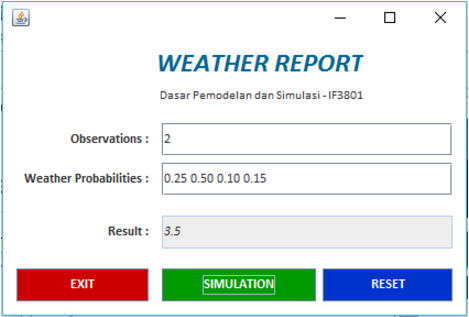
\includegraphics[width=\linewidth]{Capture3.png}
		\caption{Program Weather Report}
		\label{fig:program}
\end{figure}
\hspace*{0.3cm}Program \textit{Weather Report} diatas dibuat menggunakan bahasa java dengan tampilan GUI (\textit{Graphical User Interface}), dimana pada baris pertama merupakan jumlah observasi, lalu pada baris ke dua merupakan 4 nilai probabilitas cuaca dengan spasi sebagai pemisahnya. Nilai-nilai tersebut haruslah berjumlah sama dengan 1. Dan baris ke tiga sebagai output hasil simulasi.\\
\hspace*{0.6cm}Dari program tersebut kami melakukan 2 metode percobaan, pertama kami buat jumlah observasinya tetap namun nilai probabilitasnya berbeda-beda (pada letaknya), dan yang kedua jumlah observasinya berbeda-beda namun nilai probabilitasnya sama. Hasilnya dapat dilihat pada tabel berikut :
\begin{table}[H]
	\centering
	\caption{hasil simulasi dimana jumlah observasi tetap dan nilai probabilitasnya berbeda-beda}
	\label{sim1}
	\begin{tabular}{|c|c|c|}
		\hline
		Observasi & \begin{tabular}[c]{@{}c@{}}Probabilitas\\   Cuaca\end{tabular} & Output Simulasi \\ \hline
		5         & 0.15 0.20 0.15 0.50                                            & 8.9574225       \\ \hline
		5        & 0.50 0.20 0.15 0.15                                            & 8.9574225       \\ \hline
		5        & 0.20 0.50 0.15 0.15                                            & 8.9574225       \\ \hline
	\end{tabular}
\end{table}

\begin{table}[H]
	\centering
	\caption{hasil simulasi dimana jumlah observasi berbeda-beda dan nilai probabilitasnya sama}
	\label{sim2}
	\begin{tabular}{|c|c|c|}
		\hline
		Observasi & \begin{tabular}[c]{@{}c@{}}Probabilitas\\   Cuaca\end{tabular} & Output Simulasi    \\ \hline
		5         & 0.15 0.20 0.15 0.50                                            & 8.9574225          \\ \hline
		10        & 0.15 0.20 0.15 0.50                                             & 17.883808339171875 \\ \hline
		15        & 0.15 0.20 0.15 0.50                                             & 26.810855613654084 \\ \hline
	\end{tabular}
\end{table}
\hspace*{0.3cm}Berdasarkan kedua tabel diatas, dapat dilihat perbandingan bahwa ketika jumlah observasi yang sama namun nilai probabilitas-probabilitasnya berbeda (pada letak penginputannya) maka akan menghasilkan output yang sama. Artinya, nilai-nilai probabilitas pada setiap perkiraan cuaca yang dibangkitkan tidak terlalu berpengaruh pada jumlah bit yang dihasilkan pada proses \textit{encoding}. Namun ketika jumlah observasinya berbeda-beda dan nilai probabilitasnnya sama maka output jumlah bit yang dihasilkan akan berbeda-beda pada proses \textit{encoding}-nya.
\section{Kesimpulan}
Kesimpulan yang didapat dari hasil analisis dan simuluasi kompresi data pada laporan cuaca menggunakan metode Huffman Coding yang kami lakukan yaitu :
\begin{enumerate}
	\item Dengan algoritma huffman ini mampu memberikan penghematan pemakaian memori sampai 30\%, nilai ini didapat karena kompleksitas algoritma Huffman yaitu $O(n log n)$ untuk himpunan dengan $n$ data.
	\item Banyaknya jumlah observasi dan nilai probabilitas pada masing-masing cuaca akan menghasilkan jumlah bit data dari proses \textit{encoding} yang berbeda-beda.
	\item Pada algoritma pembentukan \textit{tree} Huffman ini, frekuensi kemunculan nilai probabilitas pada setiap observasi akan mempengaruhi panjang/jumlah bit yang dihasilkan. Semakin sering frekuensi kemunculan nilai probabilitas pada sejumlah $n$ observasi akan menghasilkan panjang/jumlah bit yang relatif sedikit. Sedangkan apabila frekuensi kemunculan nilai probabilitasnya semakin jarang, maka akan menghasilkan panjang/jumlah bit yang lebih banyak. Hal ini akan berpengaruh terhadap pemakaian memori dan efisiensi transmisi data yang dikirimkan.
\end{enumerate}
\vspace*{1cm}
\begin{thebibliography}{5}
\bibitem{1}
Gustari, Indra, Tri Wahyuni Hadi, Safwan Hadi, dan Findy Renggono. \textit{Jurnal Meteorologi dan Geofisika}
Vol. 13 No. 2: 119-130. 2012

\bibitem{2}
Hanggoro, Wido, Iis Widya Harmoko, Setyawan Widyarto.
\textit{Pendistribusian Data NWP dengan GrADS Data Server}.
Seminar Nasional Informatika. 2012.

\bibitem{3}
Rinaldi Munir.
\textit{Kompresi Teks Menggunakan Algoritma dan Pohon Huffman}. Informatika STEI ITB. 2007.
\end{thebibliography}

\end{document}


